\section{Experiments}



\subsection{Query Sources \& Generation}



\subsection{Experimental Setting}

% - Which parameters are common for all tests
% - What are the ranges/values each parameter can take.
% - Which parameters are set to a default value unless otherwise stated (and what are the default values)
% - Which methods, and in which configuration, do we consider.
% 
% SPC: level/partitions
% ALL: cacehe size
% HQF, SPC: cache type
% ALL: Map/dataset
% ALL: number of queries

Our 3 caching methods, SPC, HQF, and LRU, share a number of common settings which, unless stated otherwise, will be set to their default values: 
The number of levels in the kD-tree are 14 (i.e. 16.384 regions). We will use the list cache representation as the default cache representation, where each vertex use one byte. The default cache size is set to 5.120.000 bytes.



\subsection{Proxy}\label{subsec:expProxy}


\subsubsection{Range}

\begin{figure}[htb]
\center
  \begin{tabular}{ccc}
     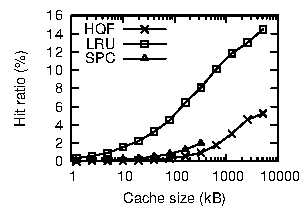
\includegraphics[width=0.5\columnwidth]{figures/cachesize_hitratio_rangenaive_aal.pdf}
     &
     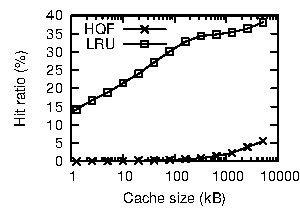
\includegraphics[width=0.5\columnwidth]{figures/cachesize_hitratio_rangenaive_bei.pdf}
      \\
     (a) Aalborg & (b)  Beijing
     \end{tabular}
\caption{Hit ratio vs. cache size, NAIVE algorithm}
\label{fig:cachesizeVsHitRatioRangeNaive}
\end{figure}

\begin{figure}[htb]
\center
  \begin{tabular}{ccc}
     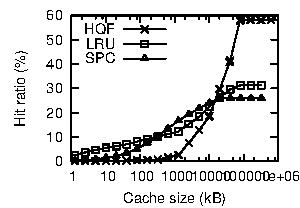
\includegraphics[width=0.5\columnwidth]{figures/cachesize_hitratio_rangefair_aal.pdf}
     &
     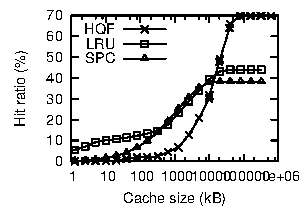
\includegraphics[width=0.5\columnwidth]{figures/cachesize_hitratio_rangefair_bei.pdf}
      \\
     (a) Aalborg & (b)  Beijing
     \end{tabular}
\caption{Hit ratio vs. cache size, FAIR algorithm}
\label{fig:cachesizeVsHitRatioRangeFair}
\end{figure}


\begin{figure}[htb]
\center
  \begin{tabular}{ccc}
     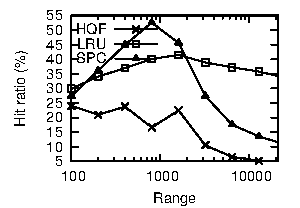
\includegraphics[width=0.5\columnwidth]{figures/range_hitratio_rangefair_aal.pdf}
     &
     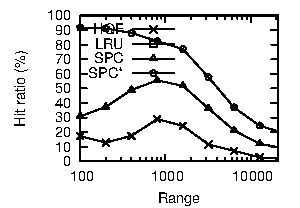
\includegraphics[width=0.5\columnwidth]{figures/range_hitratio_rangefair_bei.pdf}
      \\
     (a) Aalborg & (b)  Beijing
     \end{tabular}
\caption{Hit ratio vs. Range, FAIR algorithm}
\label{fig:rangeVsHitRatio}
\end{figure}


\subsection{Server}\label{subsec:expServer}



% \begin{figure}[htb]
% \center
%   \begin{tabular}{ccc}
%      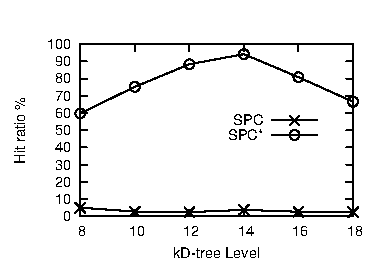
\includegraphics[width=0.5\columnwidth]{figures/aalborgHitVsLevelServer.pdf}
%      &
%      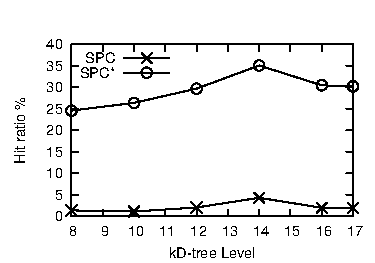
\includegraphics[width=0.5\columnwidth]{figures/beijingHitVsLevelServer.pdf}
%       \\
%      (a) Aalborg data & (b)  Beijing data
%      \end{tabular}
% \caption{Hit ratio vs. Levels}
% \label{fig:levelVsHitRatio}
% \end{figure}















% % 
% % 
% epstopdf aalborgHitVsCacheSize.eps
% epstopdf aalborgHitVsCacheSizeServer.eps
% epstopdf aalborgHitVsLevel.eps
% epstopdf aalborgHitVsLevelServer.eps
% epstopdf aalborgNodesVisitedVsCacheSize.eps
% epstopdf aalborgNodesVisitedVsLevelServer.eps
% epstopdf aalborgRuntimeVsCacheSize.eps
% epstopdf aalborgRuntimeVsLevel.eps
% epstopdf beijingHitVsCacheSize.eps
% epstopdf beijingHitVsCacheSizeServer.eps
% epstopdf beijingHitVsLevel.eps
% epstopdf beijingHitVsLevelServer.eps
% epstopdf beijingNodesVisitedVsCacheSize.eps
% epstopdf beijingNodesVisitedVsLevelServer.eps
% epstopdf beijingRuntimeVsCacheSize.eps
% epstopdf beijingRuntimeVsLevelServer.eps
% 
% load './aalborgHitVsCacheSize.p
% load './aalborgHitVsCacheSizeServer.p
% load './aalborgHitVsLevel.p
% load './aalborgHitVsLevelServer.p
% load './aalborgNodesVisitedVsCacheSize.p
% load './aalborgNodesVisitedVsLevel.p
% load './aalborgRuntimeVsCacheSize.p
% load './aalborgRuntimeVsLevel.p
% load './beijingHitVsCacheSize.p
% load './beijingHitVsCacheSizeServer.p
% load './beijingHitVsLevel.p
% load './beijingHitVsLevelServer.p
% load './beijingNodesVisitedVsCacheSize.p
% load './beijingNodesVisitedVsLevel.p
% load './beijingRuntimeVsCacheSize.p
% load './beijingRuntimeVsLevel.p
